\documentclass{standalone}
\usepackage{tikz}
\usetikzlibrary{patterns, positioning}
\usepackage[sfdefault]{ClearSans} %% option 'sfdefault' activates Clear Sans as the default text font
\usepackage[T1]{fontenc}

\begin{document}
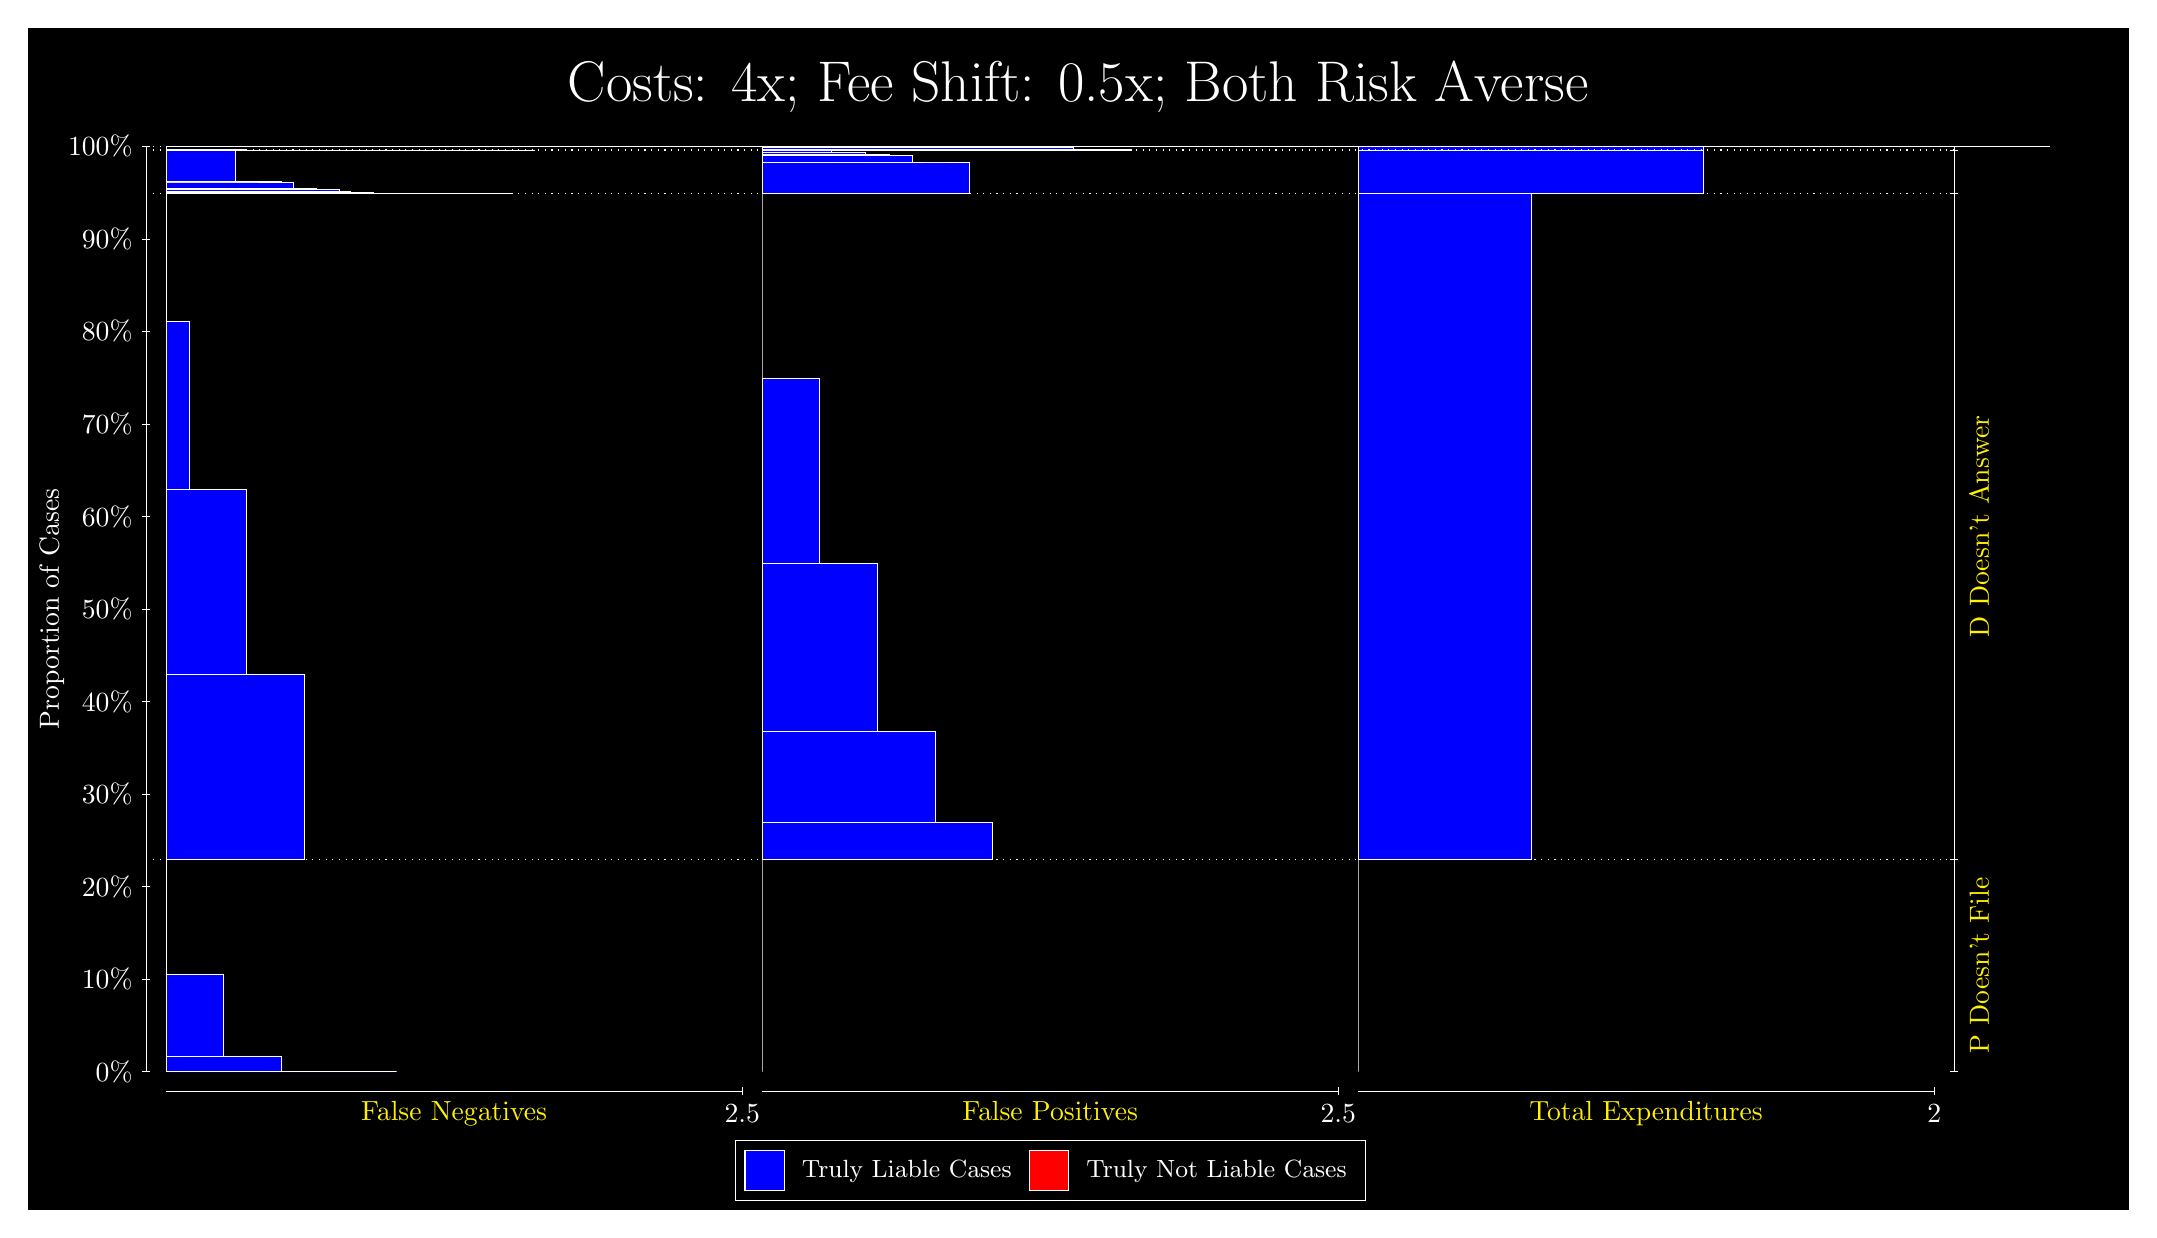
\begin{tikzpicture}
\draw[fill=black] (0,0) rectangle (26.667,15);
\draw[text=white] (0,13.5) rectangle (26.667,15) node[midway] {\huge Costs: 4x; Fee Shift: 0.5x; Both Risk Averse};
\draw[white, very thin] (1.5,1.75) -- (1.5,13.5);
\node[rotate=90, text=white, anchor=center] at (0.3, 7.625) {Proportion of Cases};
\draw[white, very thin] (1.45,1.75) -- (1.55,1.75);
\node[text=white, anchor=east] at (1.45, 1.75) {0\%};
\draw[white, very thin] (1.45,2.925) -- (1.55,2.925);
\node[text=white, anchor=east] at (1.45, 2.925) {10\%};
\draw[white, very thin] (1.45,4.1) -- (1.55,4.1);
\node[text=white, anchor=east] at (1.45, 4.1) {20\%};
\draw[white, very thin] (1.45,5.275) -- (1.55,5.275);
\node[text=white, anchor=east] at (1.45, 5.275) {30\%};
\draw[white, very thin] (1.45,6.45) -- (1.55,6.45);
\node[text=white, anchor=east] at (1.45, 6.45) {40\%};
\draw[white, very thin] (1.45,7.625) -- (1.55,7.625);
\node[text=white, anchor=east] at (1.45, 7.625) {50\%};
\draw[white, very thin] (1.45,8.8) -- (1.55,8.8);
\node[text=white, anchor=east] at (1.45, 8.8) {60\%};
\draw[white, very thin] (1.45,9.975) -- (1.55,9.975);
\node[text=white, anchor=east] at (1.45, 9.975) {70\%};
\draw[white, very thin] (1.45,11.15) -- (1.55,11.15);
\node[text=white, anchor=east] at (1.45, 11.15) {80\%};
\draw[white, very thin] (1.45,12.325) -- (1.55,12.325);
\node[text=white, anchor=east] at (1.45, 12.325) {90\%};
\draw[white, very thin] (1.45,13.5) -- (1.55,13.5);
\node[text=white, anchor=east] at (1.45, 13.5) {100\%};

\draw[white, very thin] (24.457,1.75) -- (24.457,13.5);
\draw[white, very thin] (24.407,1.75) -- (24.507,1.75);
\node[anchor=west] at (24.407, 1.75) {};
\draw[white, very thin] (24.407,4.4438) -- (24.507,4.4438);
\node[anchor=west] at (24.407, 4.4438) {};
\draw[white, very thin] (24.407,12.903) -- (24.507,12.903);
\node[anchor=west] at (24.407, 12.903) {};
\draw[white, very thin] (24.407,13.448) -- (24.507,13.448);
\node[anchor=west] at (24.407, 13.448) {};
\draw[white, very thin] (24.407,13.456) -- (24.507,13.456);
\node[anchor=west] at (24.407, 13.456) {};
\draw[white, very thin] (24.407,13.498) -- (24.507,13.498);
\node[anchor=west] at (24.407, 13.498) {};
\draw[white, very thin] (24.407,13.5) -- (24.507,13.5);
\node[anchor=west] at (24.407, 13.5) {};

\draw[white, very thin, fill=blue] (1.75,1.75) rectangle (4.6775,1.75);
\draw[white, very thin, fill=blue] (1.75,1.75) rectangle (3.9457,1.7516);
\draw[white, very thin, fill=blue] (1.75,1.7516) rectangle (3.2138,1.9385);
\draw[white, very thin, fill=blue] (1.75,1.9385) rectangle (2.4819,2.9827);
\draw[white, very thin, fill=red] (1.75,2.9827) rectangle (1.75,2.9827);
\draw[white, very thin, fill=blue] (1.75,2.9827) rectangle (1.75,4.4438);
\draw[white, very thin, fill=blue] (1.75,4.4438) rectangle (3.5065,6.7937);
\draw[white, very thin, fill=blue] (1.75,6.7937) rectangle (2.7746,9.1418);
\draw[white, very thin, fill=blue] (1.75,9.1418) rectangle (2.0428,11.274);
\draw[white, very thin, fill=red] (1.75,11.274) rectangle (1.75,11.274);
\draw[white, very thin, fill=blue] (1.75,11.274) rectangle (1.75,12.903);
\draw[white, very thin, fill=blue] (1.75,12.903) rectangle (6.1413,12.903);
\draw[white, very thin, fill=blue] (1.75,12.903) rectangle (5.8486,12.903);
\draw[white, very thin, fill=blue] (1.75,12.903) rectangle (5.5558,12.903);
\draw[white, very thin, fill=blue] (1.75,12.903) rectangle (5.4094,12.903);
\draw[white, very thin, fill=blue] (1.75,12.903) rectangle (5.1167,12.903);
\draw[white, very thin, fill=blue] (1.75,12.903) rectangle (4.8239,12.903);
\draw[white, very thin, fill=blue] (1.75,12.903) rectangle (4.6775,12.904);
\draw[white, very thin, fill=blue] (1.75,12.904) rectangle (4.3848,12.921);
\draw[white, very thin, fill=blue] (1.75,12.921) rectangle (4.092,12.928);
\draw[white, very thin, fill=blue] (1.75,12.928) rectangle (3.9457,12.949);
\draw[white, very thin, fill=blue] (1.75,12.949) rectangle (3.6529,12.967);
\draw[white, very thin, fill=blue] (1.75,12.967) rectangle (3.3602,13.049);
\draw[white, very thin, fill=blue] (1.75,13.049) rectangle (3.2138,13.05);
\draw[white, very thin, fill=blue] (1.75,13.05) rectangle (2.921,13.05);
\draw[white, very thin, fill=blue] (1.75,13.05) rectangle (2.6283,13.448);
\draw[white, very thin, fill=red] (1.75,13.448) rectangle (1.75,13.448);
\draw[white, very thin, fill=blue] (1.75,13.448) rectangle (6.4341,13.448);
\draw[white, very thin, fill=blue] (1.75,13.448) rectangle (5.7022,13.448);
\draw[white, very thin, fill=blue] (1.75,13.448) rectangle (4.9703,13.448);
\draw[white, very thin, fill=blue] (1.75,13.448) rectangle (4.2384,13.456);
\draw[white, very thin, fill=blue] (1.75,13.456) rectangle (3.5065,13.456);
\draw[white, very thin, fill=red] (1.75,13.456) rectangle (1.75,13.456);
\draw[white, very thin, fill=blue] (1.75,13.456) rectangle (3.5065,13.456);
\draw[white, very thin, fill=blue] (1.75,13.456) rectangle (2.7746,13.457);
\draw[white, very thin, fill=blue] (1.75,13.457) rectangle (2.0428,13.463);
\draw[white, very thin, fill=red] (1.75,13.463) rectangle (1.75,13.463);
\draw[white, very thin, fill=blue] (1.75,13.463) rectangle (1.75,13.498);
\draw[white, very thin, fill=blue] (1.75,13.498) rectangle (9.9471,13.498);
\draw[white, very thin, fill=blue] (1.75,13.498) rectangle (9.2152,13.498);
\draw[white, very thin, fill=blue] (1.75,13.498) rectangle (8.4834,13.498);
\draw[white, very thin, fill=blue] (1.75,13.498) rectangle (7.7515,13.498);
\draw[white, very thin, fill=blue] (1.75,13.498) rectangle (7.0196,13.499);
\draw[white, very thin, fill=blue] (1.75,13.499) rectangle (6.2877,13.499);
\draw[white, very thin, fill=blue] (1.75,13.499) rectangle (5.7022,13.499);
\draw[white, very thin, fill=blue] (1.75,13.499) rectangle (4.9703,13.499);
\draw[white, very thin, fill=blue] (1.75,13.499) rectangle (4.2384,13.499);
\draw[white, very thin, fill=blue] (1.75,13.499) rectangle (3.5065,13.5);
\draw[white, very thin, fill=blue] (1.75,13.5) rectangle (2.7746,13.5);
\draw[white, very thin, fill=blue] (1.75,13.5) rectangle (2.0428,13.5);
\draw[white, very thin, fill=red] (1.75,13.5) rectangle (1.75,13.5);
\draw[white, very thin, fill=blue] (1.75,13.5) rectangle (1.75,13.5);
\draw[white, very thin, fill=red] (9.3189,1.75) rectangle (9.3189,1.75);
\draw[white, very thin, fill=blue] (9.3189,1.75) rectangle (9.3189,4.4438);
\draw[white, very thin, fill=red] (9.3189,4.4438) rectangle (12.246,4.4438);
\draw[white, very thin, fill=blue] (9.3189,4.4438) rectangle (12.246,4.9212);
\draw[white, very thin, fill=blue] (9.3189,4.9212) rectangle (11.515,6.0733);
\draw[white, very thin, fill=blue] (9.3189,6.0733) rectangle (10.783,8.2051);
\draw[white, very thin, fill=blue] (9.3189,8.2051) rectangle (10.051,10.553);
\draw[white, very thin, fill=blue] (9.3189,10.553) rectangle (9.3189,12.903);
\draw[white, very thin, fill=red] (9.3189,12.903) rectangle (11.954,12.903);
\draw[white, very thin, fill=blue] (9.3189,12.903) rectangle (11.954,13.301);
\draw[white, very thin, fill=red] (9.3189,13.301) rectangle (11.661,13.301);
\draw[white, very thin, fill=blue] (9.3189,13.301) rectangle (11.661,13.301);
\draw[white, very thin, fill=red] (9.3189,13.301) rectangle (11.368,13.301);
\draw[white, very thin, fill=blue] (9.3189,13.301) rectangle (11.368,13.302);
\draw[white, very thin, fill=blue] (9.3189,13.302) rectangle (11.222,13.385);
\draw[white, very thin, fill=blue] (9.3189,13.385) rectangle (10.929,13.402);
\draw[white, very thin, fill=blue] (9.3189,13.402) rectangle (10.636,13.424);
\draw[white, very thin, fill=blue] (9.3189,13.424) rectangle (10.49,13.43);
\draw[white, very thin, fill=blue] (9.3189,13.43) rectangle (10.197,13.447);
\draw[white, very thin, fill=blue] (9.3189,13.447) rectangle (9.9044,13.448);
\draw[white, very thin, fill=blue] (9.3189,13.448) rectangle (9.758,13.448);
\draw[white, very thin, fill=blue] (9.3189,13.448) rectangle (9.4652,13.448);
\draw[white, very thin, fill=blue] (9.3189,13.448) rectangle (9.3189,13.448);
\draw[white, very thin, fill=red] (9.3189,13.448) rectangle (11.075,13.448);
\draw[white, very thin, fill=blue] (9.3189,13.448) rectangle (11.075,13.449);
\draw[white, very thin, fill=blue] (9.3189,13.449) rectangle (10.344,13.456);
\draw[white, very thin, fill=blue] (9.3189,13.456) rectangle (9.6116,13.456);
\draw[white, very thin, fill=blue] (9.3189,13.456) rectangle (9.3189,13.456);
\draw[white, very thin, fill=red] (9.3189,13.456) rectangle (14.003,13.456);
\draw[white, very thin, fill=blue] (9.3189,13.456) rectangle (14.003,13.468);
\draw[white, very thin, fill=blue] (9.3189,13.468) rectangle (13.271,13.491);
\draw[white, very thin, fill=blue] (9.3189,13.491) rectangle (12.539,13.497);
\draw[white, very thin, fill=blue] (9.3189,13.497) rectangle (11.807,13.498);
\draw[white, very thin, fill=blue] (9.3189,13.498) rectangle (11.075,13.498);
\draw[white, very thin, fill=red] (9.3189,13.498) rectangle (17.516,13.498);
\draw[white, very thin, fill=blue] (9.3189,13.498) rectangle (17.516,13.498);
\draw[white, very thin, fill=red] (9.3189,13.498) rectangle (16.784,13.498);
\draw[white, very thin, fill=blue] (9.3189,13.498) rectangle (16.784,13.498);
\draw[white, very thin, fill=red] (9.3189,13.498) rectangle (16.052,13.498);
\draw[white, very thin, fill=blue] (9.3189,13.498) rectangle (16.052,13.498);
\draw[white, very thin, fill=red] (9.3189,13.498) rectangle (15.32,13.498);
\draw[white, very thin, fill=blue] (9.3189,13.498) rectangle (15.32,13.498);
\draw[white, very thin, fill=blue] (9.3189,13.498) rectangle (14.588,13.498);
\draw[white, very thin, fill=blue] (9.3189,13.498) rectangle (13.857,13.498);
\draw[white, very thin, fill=blue] (9.3189,13.498) rectangle (13.125,13.498);
\draw[white, very thin, fill=blue] (9.3189,13.498) rectangle (12.393,13.498);
\draw[white, very thin, fill=red] (9.3189,13.498) rectangle (11.807,13.498);
\draw[white, very thin, fill=blue] (9.3189,13.498) rectangle (11.807,13.499);
\draw[white, very thin, fill=red] (9.3189,13.499) rectangle (11.075,13.499);
\draw[white, very thin, fill=blue] (9.3189,13.499) rectangle (11.075,13.5);
\draw[white, very thin, fill=blue] (9.3189,13.5) rectangle (10.344,13.5);
\draw[white, very thin, fill=blue] (9.3189,13.5) rectangle (9.6116,13.5);
\draw[white, very thin, fill=blue] (9.3189,13.5) rectangle (9.3189,13.5);
\draw[white, very thin, fill=red] (16.888,1.75) rectangle (16.888,1.75);
\draw[white, very thin, fill=blue] (16.888,1.75) rectangle (16.888,4.4438);
\draw[white, very thin, fill=red] (16.888,4.4438) rectangle (19.083,4.4438);
\draw[white, very thin, fill=blue] (16.888,4.4438) rectangle (19.083,12.903);
\draw[white, very thin, fill=red] (16.888,12.903) rectangle (21.279,12.903);
\draw[white, very thin, fill=blue] (16.888,12.903) rectangle (21.279,13.448);
\draw[white, very thin, fill=red] (16.888,13.448) rectangle (21.279,13.448);
\draw[white, very thin, fill=blue] (16.888,13.448) rectangle (21.279,13.456);
\draw[white, very thin, fill=red] (16.888,13.456) rectangle (21.279,13.456);
\draw[white, very thin, fill=blue] (16.888,13.456) rectangle (21.279,13.498);
\draw[white, very thin, fill=red] (16.888,13.498) rectangle (25.67,13.498);
\draw[white, very thin, fill=blue] (16.888,13.498) rectangle (25.67,13.5);
\draw[white, dotted] (1.5,4.4438) -- (24.457,4.4438);
\draw[white, dotted] (1.5,12.903) -- (24.457,12.903);
\draw[white, dotted] (1.5,13.448) -- (24.457,13.448);
\draw[white, dotted] (1.5,13.456) -- (24.457,13.456);
\draw[white, dotted] (1.5,13.498) -- (24.457,13.498);
\draw[white, very thin] (1.75,1.5) -- (9.0689,1.5);
\node[text=yellow, anchor=north] at (5.4094, 1.5) {False Negatives};
\draw[white, very thin] (9.0689,1.45) -- (9.0689,1.55);
\node[text=white, anchor=north] at (9.0689, 1.45) {2.5};

\draw[white, very thin] (9.3189,1.5) -- (16.638,1.5);
\node[text=yellow, anchor=north] at (12.978, 1.5) {False Positives};
\draw[white, very thin] (16.638,1.45) -- (16.638,1.55);
\node[text=white, anchor=north] at (16.638, 1.45) {2.5};

\draw[white, very thin] (16.888,1.5) -- (24.207,1.5);
\node[text=yellow, anchor=north] at (20.547, 1.5) {Total Expenditures};
\draw[white, very thin] (24.207,1.45) -- (24.207,1.55);
\node[text=white, anchor=north] at (24.207, 1.45) {2};

\node[text=yellow, centered, rotate=90] at (24.777, 3.0969) {P Doesn't File};
\node[text=yellow, centered, rotate=90] at (24.777, 8.6735) {D Doesn't Answer};





\draw (12.978300999999998,1.5) node[draw=none] (baseCoordinate) {};
\begin{scope}[align=center]
        \matrix[scale=0.5, draw=white, below=0.5cm of baseCoordinate, nodes={draw}, column sep=0.1cm]{
            \node[rectangle, draw, minimum width=0.5cm, minimum height=0.5cm, fill=blue] {}; &
            \node[draw=none, font=\small, text=white] (B) {Truly Liable Cases}; &
            \node[rectangle, draw, minimum width=0.5cm, minimum height=0.5cm, fill=red] {}; &
            \node[draw=none, font=\small, text=white] (B) {Truly Not Liable Cases}; \\
            };
\end{scope}

\end{tikzpicture}
\end{document}